\documentclass[fontscale=0.38,a0paper]{baposter}

\tracingstats=2

\usepackage{times}
\usepackage{calc}
\usepackage{graphicx}
\usepackage{amsmath}
\usepackage{amssymb}
\usepackage{relsize}
\usepackage{multirow}
\usepackage{bm}
\usepackage{caption}
\usepackage[authoryear,round]{natbib}
\usepackage[hidelinks]{hyperref}

\usepackage{tabularx}
\usepackage{booktabs}

\usepackage{colortbl}

\usepackage{multicol}

%\usepackage{pgfbaselayers}
%\pgfdeclarelayer{background}
%\pgfdeclarelayer{foreground}
%\pgfsetlayers{background,main,foreground}


%\usepackage{tikz}
%\usetikzlibrary{arrows,backgrounds,patterns,matrix,shapes,fit,calc,shadows,plotmarks,decorations.pathmorphing,positioning,trees}

\renewcommand{\familydefault}{\sfdefault}
\usepackage{helvet}
\usepackage{bookman}
\usepackage{palatino}

% My stuff
\newcommand{\R}{\mathbb{R}}
\newcommand{\E}{\mathbb{E}}
\renewcommand{\P}{\mathbb{P}}
\newcommand{\st}{\,\colon\,}
\newcommand{\bone}{\mathbf{1}}
\newcommand{\var}{\mathop{\mbox{Var}}}
\newcommand{\cov}{\mathop{\mbox{cov}}}
\newcommand{\tskit}{{\texttt{tskit}}}
\newcommand{\branch}{\mbox{Branch}} % branch stat
\newcommand{\branchp}{\mbox{Branch}_+} % polarised
\newcommand{\site}{\mbox{Site}} % site stat
\newcommand{\sitep}{\mbox{Site}_+} % polarised
\newcommand{\node}{\mbox{Node}} % node stat
\newcommand{\nodep}{\mbox{Node}_+} % polarised
\newcommand{\given}{\;\vert\;}

\newcommand{\treeseq}{\mathbb{T}} % tree sequence
\newcommand{\iw}{w} % sample (initial) weights
\newcommand{\tiw}{w_\text{total}} % total sample (initial) weights
\newcommand{\nw}{x} % subtree (node) weights
\newcommand{\aw}{{\bar x}} % allele weights


% end my stuff

\selectcolormodel{cmyk}

% \graphicspath{{images/}}

%%%%%%%%%%%%%%%%%%%%%%%%%%%%%%%%%%%%%%%%%%%%%%%%%%%%%%%%%%%%%%%%%%%%%%%%%%%%%%%%
%%%% Some symbols used in the text
%%%%%%%%%%%%%%%%%%%%%%%%%%%%%%%%%%%%%%%%%%%%%%%%%%%%%%%%%%%%%%%%%%%%%%%%%%%%%%%%
%\newcommand{\sub}[2]{\ensuremath{#1_{\textrm{#2}}}}
%\newcommand{\gen}[2]{\ensuremath{\textrm{#1}_{\textrm{#2}}}}


%%%%%%%%%%%%%%%%%%%%%%%%%%%%%%%%%%%%%%%%%%%%%%%%%%%%%%%%%%%%%%%%%%%%%%%%%%%%%%%%
% Multicol Settings
%%%%%%%%%%%%%%%%%%%%%%%%%%%%%%%%%%%%%%%%%%%%%%%%%%%%%%%%%%%%%%%%%%%%%%%%%%%%%%%%
\setlength{\columnsep}{1em}
\setlength{\columnseprule}{0mm} % no vertical line


%%%%%%%%%%%%%%%%%%%%%%%%%%%%%%%%%%%%%%%%%%%%%%%%%%%%%%%%%%%%%%%%%%%%%%%%%%%%%%%%
% Save space in lists. Use this after the opening of the list
%%%%%%%%%%%%%%%%%%%%%%%%%%%%%%%%%%%%%%%%%%%%%%%%%%%%%%%%%%%%%%%%%%%%%%%%%%%%%%%%
\newcommand{\compresslist}{
\setlength{\itemsep}{1pt}
\setlength{\parskip}{0pt}
\setlength{\parsep}{0pt}
}

%%%%%%%%%%%%%%%%%%%%%%%%%%%%%%%%%%%%%%%%%%%%%%%%%%%%%%%%%%%%%%%%%%%%%%%%%%%%%%
%%% Other Macros
%%%%%%%%%%%%%%%%%%%%%%%%%%%%%%%%%%%%%%%%%%%%%%%%%%%%%%%%%%%%%%%%%%%%%%%%%%%%%%
% \renewcommand{\labelenumi}{\alph{enumi})}
% \renewcommand{\theenumi}{\alph{enumi})}
\newcommand{\postercaption}[1]{\begin{minipage}{\linewidth}\center\smaller
  {#1}\end{minipage}}



%%%%%%%%%%%%%%%%%%%%%%%%%%%%%%%%%%%%%%%%%%%%%%%%%%%%%%%%%%%%%%%%%%%%%%%%%%%%%%
%%% Begin of Document
%%%%%%%%%%%%%%%%%%%%%%%%%%%%%%%%%%%%%%%%%%%%%%%%%%%%%%%%%%%%%%%%%%%%%%%%%%%%%%

\begin{document}

%%%%%%%%%%%%%%%%%%%%%%%%%%%%%%%%%%%%%%%%%%%%%%%%%%%%%%%%%%%%%%%%%%%%%%%%%%%%%%
%%% Here starts the poster
%%%---------------------------------------------------------------------------
%%% Format it to your taste with the options
%%%%%%%%%%%%%%%%%%%%%%%%%%%%%%%%%%%%%%%%%%%%%%%%%%%%%%%%%%%%%%%%%%%%%%%%%%%%%%

% Define some colors
\definecolor{silver}{cmyk}{0,0,0,0.3}
\definecolor{black}{cmyk}{0,0,0.0,1.0}
\definecolor{white}{cmyk}{0,0,0.0,0.0}
\definecolor{darkSilver}{cmyk}{0,0,0,0.1}

\definecolor{darkYellow}{cmyk}{0,0,1.0,0.5}
\definecolor{yellow}{cmyk}{0,0,0.9,0.0}
\definecolor{reddishyellow}{cmyk}{0,0.22,1.0,0.0}
\definecolor{lightyellow}{cmyk}{0,0,0.3,0.0}
\definecolor{lighteryellow}{cmyk}{0,0,0.1,0.0}
\definecolor{lightestyellow}{cmyk}{0,0,0.05,0.0}

\definecolor{DavisBlue}{cmyk}{1,0.56,0,0.34}
%    C = 100  M = 56  Y = 0 K = 34


\definecolor{HohenheimBlue}{cmyk}{1,0.5,0,0.45}
\definecolor{HohenheimLightLightBlue}{RGB}{243,250,255}
\definecolor{HohenheimLightBlue}{RGB}{215,221,235}
\definecolor{HohenheimDarkBlue}{RGB}{52,104,152}
\definecolor{darkCyan}{cmyk}{1,1,0,0.5}
\definecolor{cyan}{cmyk}{1,0,0,0.0}
\definecolor{lightcyan}{cmyk}{0.3,0,0,0.0}
\definecolor{lightercyan}{cmyk}{0.1,0,0,0.0}
\definecolor{lightestcyan}{cmyk}{0.05,0,0,0.0}



\typeout{Poster Starts}
%Define custom background
\background{
  \begin{tikzpicture}[remember picture,overlay]%
    \draw (current page.north west)+(-2em,2em) node[anchor=north west] {\includegraphics[height=\textheight]{silhouettes_background}};
  \end{tikzpicture}%
}

\newlength{\leftimgwidth}
\begin{poster}%
  % Poster Options
  {
  % Columns and Column spacing
  columns=3,
  colspacing=1.5em,
  % Background
  % background=user,
  background=shade-tb,
  % Poster header options
  eyecatcher=yes,
  posterheaderheight=0.15\textheight,
  % Format of textbox header
  headerborder=open,
  % headershape=small-rounded,
  headershape=roundedright,
  headershade=shade-tb,
  % headershade=plain,
  headerfont=\Large\textsf, %Sans Serif
  % Format of textbox
  boxborder=small-rounded,
  % boxborder=roundedleft,    
  boxshade=plain,
  linewidth=0.5pt,
  % Color style
  % bgColorOne=lightestcyan,
  % bgColorTwo=lightcyan,
  bgColorOne=white,
  bgColorTwo=white,
  % borderColor=cyan,
  borderColor=black,
  headerColorOne=DavisBlue,
  % headerColorOne=cyan,
  headerColorTwo=black,
  % headerFontColor=black,
  headerFontColor=white,
  % boxColorOne=lightercyan,
  boxColorOne=HohenheimLightLightBlue,
  boxColorTwo=white,
  % Show grid to help with alignment
  grid=no
  % grid=yes
  }
  % Eye Catcher
  {
  \makebox[15em][r]{%
    \begin{minipage}{15em}
       \hfill
       
\includegraphics[width=15em]{tskit_logo} \\
    \end{minipage}
    }
  }
  % Title
  {\sf %Sans Serif
  %\bf% %bold  
  \vspace{0.5em}
     \textbf{\textcolor{DavisBlue}{Fast computation and duality \\ for tree sequence statistics}}\vspace{0.5em}}
  % Authors
  {\sf %Sans Serif
    Peter Ralph$^{\ddagger}$, Kevin Thornton$^{\dagger}$, and Jerome Kelleher$^{\S}$ \\  \vspace{-1.0mm}
    {\small \textit{$\ddagger$ Mathematics and Biology, University of Oregon} }\\ \vspace{-0.5em}
    {\small \textit{$\dagger$ Ecology \& Evolutionary Biology, UC Irvine} }\\ \vspace{-0.5em}
    {\small \textit{$\S$ Big Data Institute, University of Oxford} }\\ \vspace{0.5em}
    {\textbf{paper:}  \citep{ralph2019efficiently} } % \url{https://www.biorxiv.org/content/10.1101/779132v1} }
    {\textbf{code:}  \url{https://github.com/tskit-dev} } %\\
  }
  % Project logo
  {
    \makebox[15em][r]{%
      \begin{minipage}{12em}
        \hfill
          
\includegraphics[width=10em]{UOSignature-STK-BLK} \\
      \end{minipage}
    }
  }

  % Width of left inset image
%  \setlength{\leftimgwidth}{0.78em+0.0em}

%%%%%%%%%%%%%%%%%%%%%%%%%%%%%%%%%%%%%%%%%%%%%%%%%%%%%%%%%%%%%%%%%%%%%%%%%%%%%%
%%% Now define the boxes that make up the poster
%%%---------------------------------------------------------------------------
%%% Each box has a name and can be placed absolutely or relatively.
%%% The only inconvenience is that you can only specify a relative position 
%%% towards an already declared box. So if you have a box attached to the 
%%% bottom, one to the top and a third one which should be in between, you 
%%% have to specify the top and bottom boxes before you specify the middle 
%%% box.
%%%%%%%%%%%%%%%%%%%%%%%%%%%%%%%%%%%%%%%%%%%%%%%%%%%%%%%%%%%%%%%%%%%%%%%%%%%%%%

%%%%%%%%%%%%%%%%%%%%%%%%%%%%%%%%%%%%%%%%%%%%%%%%%%%%%%%%%%%%%%%%%%%%%%%%%%%%%%
\headerbox{Tree sequences: all the genealogies}{name=intro,column=0,row=0,span=1}{
%%%%%%%%%%%%%%%%%%%%%%%%%%%%%%%%%%%%%%%%%%%%%%%%%%%%%%%%%%%%%%%%%%%%%%%%%%%%%%

A \textbf{tree sequence} describes
a correlated sequence of genealogical trees
describing how a set of chromosomes are related.

\begin{itemize}

    \item The \emph{pedigree} plus crossover locations
        would give us the tree sequence for \emph{everyone, ever}.

    \item Much less fully describes the history of a \emph{sample} of genomes.

    \item Almost the Ancestral Recombination Graph (ARG).

\end{itemize}


\citet{kelleher2016efficient}
introduced the \textbf{succinct tree sequence} data structure
for \texttt{msprime}; it was updated in \citet{kelleher2018efficient}.

}
%%%%%%%%%%%%%%%%%%%%%%%%%%%%%%%%%%%%%%%%%%%%%%%%%%%%%%%%%%%%%%%%%%%%%%%%%%%%%%


%%%%%%%%%%%%%%%%%%%%%%%%%%%%%%%%%%%%%%%%%%%%%%%%%%%%%%%%%%%%%%%%%%%%%%%%%%%%%%
\headerbox{Tables: a data structure for tree sequences}{name=tables,column=0,span=1,below=intro}{
%%%%%%%%%%%%%%%%%%%%%%%%%%%%%%%%%%%%%%%%%%%%%%%%%%%%%%%%%%%%%%%%%%%%%%%%%%%%%%

    % We updated and generalized the data structure in \citet{kelleher2018efficient}:

    \begin{itemize}
            \compresslist

        \item \textbf{Edges:}   Who inherits from who. \\
            \emph{Records:} interval (left, right); parent node; child node.

        \item \textbf{Nodes:}   The ancestors those happen in. \\
            \emph{Records:} time ago (of birth); individual.

        \item \textbf{Mutations:}   When state changes along the tree. \\
            \emph{Records:} site index; node index; derived state.

        \item \textbf{Sites:}   Where mutations fall on the genome. \\
            \emph{Records:} genomic position; root state.

        \item \textbf{Individuals:} Optional. Containers for polyploids. \\
            \emph{Records:} metadata; pointed to by nodes.

    \end{itemize}

    % \begin{center}
    %     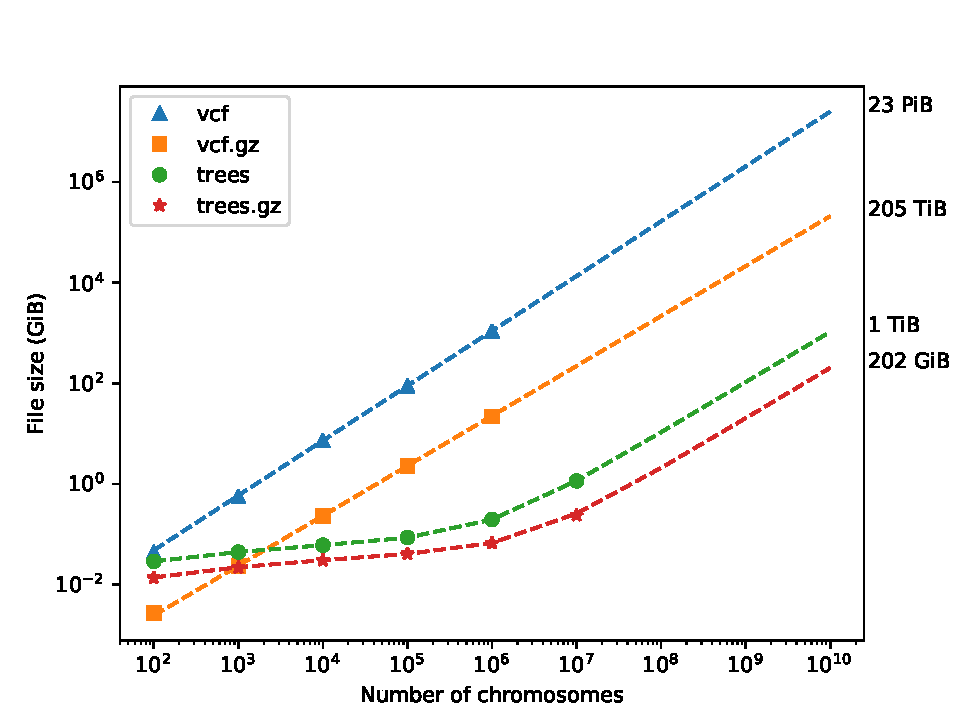
\includegraphics[width=0.75\textwidth]{storing_everyone}
    % \end{center}

}
%%%%%%%%%%%%%%%%%%%%%%%%%%%%%%%%%%%%%%%%%%%%%%%%%%%%%%%%%%%%%%%%%%%%%%%%%%%%%%


%%%%%%%%%%%%%%%%%%%%%%%%%%%%%%%%%%%%%%%%%%%%%%%%%%%%%%%%%%%%%%%%%%%%%%%%%%%%%%
\headerbox{Example}{name=ex,column=0,below=tables}{
%%%%%%%%%%%%%%%%%%%%%%%%%%%%%%%%%%%%%%%%%%%%%%%%%%%%%%%%%%%%%%%%%%%%%%%%%%%%%%

    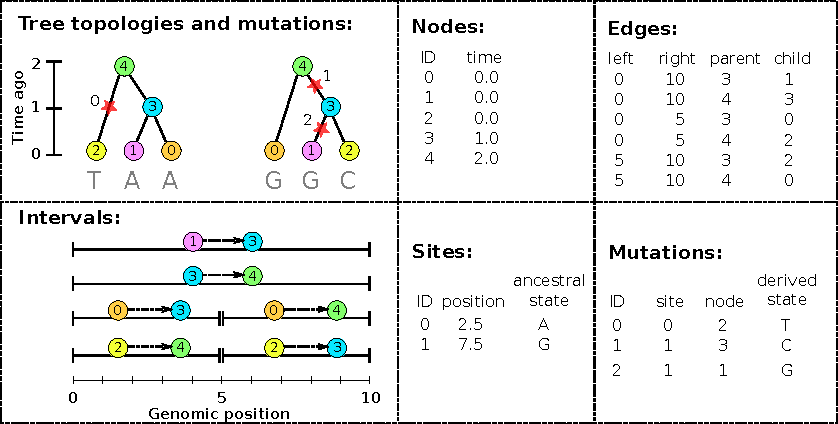
\includegraphics[width=\textwidth]{example_tree_sequence}

}

%%%%%%%%%%%%%%%%%%%%%%%%%%%%%%%%%%%%%%%%%%%%%%%%%%%%%%%%%%%%%%%%%%%%%%%%%%%%%%
\headerbox{References}{name=contrib,column=0,below=ex}{
%%%%%%%%%%%%%%%%%%%%%%%%%%%%%%%%%%%%%%%%%%%%%%%%%%%%%%%%%%%%%%%%%%%%%%%%%%%%%%
  % \scriptsize
  \renewcommand{\section}[2]{\vskip 0.0em}
  \bibliographystyle{abbrvnat}
  \setlength{\bibsep}{0.0pt}
  \bibliography{refs}
}
%%%%%%%%%%%%%%%%%%%%%%%%%%%%%%%%%%%%%%%%%%%%%%%%%%%%%%%%%%%%%%%%%%%%%%%%%%%%%%

%%%%%%%%%%%%%%%%%%%%%%%%%%%%%%%%%%%%%%%%%%%%%%%%%%%%%%%%%%%%%%%%%%%%%%%%%%%%%%

%%%%%%%%%%%%%%%%%%%%%%%%%%%%%%%%%%%%%%%%%%%%%%%%%%%%%%%%%%%%%%%%%%%%%%%%%%%%%%
\headerbox{Another example}{name=ex2,column=0,below=contrib}{
%%%%%%%%%%%%%%%%%%%%%%%%%%%%%%%%%%%%%%%%%%%%%%%%%%%%%%%%%%%%%%%%%%%%%%%%%%%%%%

    \noindent
    \tiny
\hfill
\begin{tabular}{|rr|}
  \hline
    \textbf{Nodes:} & \\
id & time \\ 
  \hline
  0 & 0.00 \\ 
    1 & 0.00 \\ 
    2 & 0.00 \\ 
    3 & 0.00 \\ 
    4 & 0.00 \\ 
    5 & 0.00 \\ 
    6 & 0.00 \\ 
    7 & 0.00 \\ 
    8 & 0.09 \\ 
    9 & 0.31 \\ 
   10 & 0.39 \\ 
   11 & 0.41 \\ 
   12 & 0.43 \\ 
   13 & 0.97 \\ 
   14 & 1.04 \\ 
   15 & 1.21 \\ 
   16 & 1.36 \\ 
   17 & 1.45 \\ 
   18 & 2.41 \\ 
   19 & 2.46 \\ 
   20 & 2.85 \\ 
   21 & 3.84 \\ 
   22 & 4.45 \\ 
   \hline
\end{tabular}
\hfill
\begin{tabular}{|rrrr|}
  \hline
    \textbf{Edges:} & & & \\
left & right & parent & child \\ 
  \hline
0.00 & 1.00 &   8 &   2 \\ 
  0.00 & 1.00 &   8 &   6 \\ 
  0.00 & 1.00 &   9 &   5 \\ 
  0.00 & 1.00 &   9 &   7 \\ 
  0.00 & 1.00 &  10 &   3 \\ 
  0.00 & 1.00 &  10 &   8 \\ 
  0.00 & 1.00 &  11 &   0 \\ 
  0.00 & 1.00 &  11 &   1 \\ 
  0.00 & 1.00 &  12 &   9 \\ 
  0.00 & 1.00 &  12 &  10 \\ 
  0.99 & 1.00 &  13 &   4 \\ 
  0.99 & 1.00 &  13 &  12 \\ 
  0.00 & 0.19 &  14 &  11 \\ 
  0.00 & 0.19 &  14 &  12 \\ 
  0.93 & 0.99 &  15 &   4 \\ 
  0.93 & 1.00 &  15 &  11 \\ 
  0.99 & 1.00 &  15 &  13 \\ 
  0.30 & 0.54 &  16 &   4 \\ 
  0.91 & 0.93 &  16 &   4 \\ 
  0.30 & 0.54 &  16 &  11 \\ 
  0.91 & 0.93 &  16 &  11 \\ 
  0.54 & 0.69 &  17 &   4 \\ 
   \hline
\end{tabular}
\begin{tabular}{|rrrr|}
  \hline
    \textbf{cont'd} & ... &  ... & ... \\
left & right & parent & child \\ 
  \hline
  0.54 & 0.69 &  17 &  12 \\ 
  0.69 & 0.91 &  18 &   4 \\ 
  0.69 & 0.91 &  18 &  11 \\ 
  0.00 & 0.30 &  19 &   4 \\ 
  0.69 & 0.69 &  19 &  11 \\ 
  0.19 & 0.46 &  19 &  12 \\ 
  0.69 & 0.99 &  19 &  12 \\ 
  0.00 & 0.19 &  19 &  14 \\ 
  0.93 & 0.99 &  19 &  15 \\ 
  0.30 & 0.46 &  19 &  16 \\ 
  0.91 & 0.93 &  19 &  16 \\ 
  0.69 & 0.69 &  19 &  17 \\ 
  0.69 & 0.91 &  19 &  18 \\ 
  0.19 & 0.30 &  20 &  11 \\ 
  0.19 & 0.30 &  20 &  19 \\ 
  0.60 & 0.69 &  21 &  11 \\ 
  0.60 & 0.69 &  21 &  17 \\ 
  0.54 & 0.60 &  22 &  11 \\ 
  0.46 & 0.54 &  22 &  12 \\ 
  0.46 & 0.54 &  22 &  16 \\ 
  0.54 & 0.60 &  22 &  17 \\ 
   \hline
\end{tabular}

}
%%%%%%%%%%%%%%%%%%%%%%%%%%%%%%%%%%%%%%%%%%%%%%%%%%%%%%%%%%%%%%%%%%%%%%%%%%%%%%




%%%%%%%%%%%%%%%%%%%%%%%%%%%%%%%%%%%%%%%%%%%%%%%%%%%%%%%%%%%%%%%%%%%%%%%%%%%%%%
\headerbox{Sample weights and summary functions}{name=weights,column=1,row=0}{
%%%%%%%%%%%%%%%%%%%%%%%%%%%%%%%%%%%%%%%%%%%%%%%%%%%%%%%%%%%%%%%%%%%%%%%%%%%%%%

A list of \textbf{sample weights} $\iw$ assigns a numeric value $\iw(v) \in \R^k$
to every sample node.

The \textbf{subtree weight} $\nw_T(u)$ on tree $T$ of node $u$
is the sum of weights of all sample nodes descended from $u$:
\begin{align*}
    \nw_T(u) = \sum_{v \,:\, v \le_T u} \iw(v) ,
\end{align*}
where $v \le_T u$ if $u$ is on the path from $v$ to root in the tree $T$.
The \textbf{total weight} is the sum of the weights over all samples:
$\tiw = \sum_v \iw(v)$.

A \textbf{summary function} is a real-valued function $f(w_1, \ldots, w_k)$
with the property that $f(0) = f(\tiw) = 0$.

}
%%%%%%%%%%%%%%%%%%%%%%%%%%%%%%%%%%%%%%%%%%%%%%%%%%%%%%%%%%%%%%%%%%%%%%%%%%%%%%


%%%%%%%%%%%%%%%%%%%%%%%%%%%%%%%%%%%%%%%%%%%%%%%%%%%%%%%%%%%%%%%%%%%%%%%%%%%%%%
\headerbox{Site statistics}{name=site,column=1,below=weights}{
%%%%%%%%%%%%%%%%%%%%%%%%%%%%%%%%%%%%%%%%%%%%%%%%%%%%%%%%%%%%%%%%%%%%%%%%%%%%%%

    The \textbf{allele weight} for allele $a$ at site $j$ is the total weight
    of all samples inheriting this allele:
    \begin{align*}
        \aw_j(a) = \sum_{v \st g_j(v) = a} \iw(v) ,
    \end{align*}
    where the sum is over all sample nodes $v$ for which
    $g_j(v)$, the allele carried by node $v$ at site $j$, is equal to $a$.

The \textbf{site statistic} at site $j$:
\begin{align}
    \site(f, \iw)_j
    &=
    \sum_{a} f(\aw_j(a)),
\end{align}
and in the \emph{window} $[i,j)$:
\begin{align}
    \site(f, \iw)_{[i,j)}
    &=
    \frac{1}{j-i} \sum_{k=i}^{j-1} \site(f, \iw)_k .
\end{align}



}
%%%%%%%%%%%%%%%%%%%%%%%%%%%%%%%%%%%%%%%%%%%%%%%%%%%%%%%%%%%%%%%%%%%%%%%%%%%%%%


%%%%%%%%%%%%%%%%%%%%%%%%%%%%%%%%%%%%%%%%%%%%%%%%%%%%%%%%%%%%%%%%%%%%%%%%%%%%%%
\headerbox{Branch statistics}{name=branch,column=1,below=site}{
%%%%%%%%%%%%%%%%%%%%%%%%%%%%%%%%%%%%%%%%%%%%%%%%%%%%%%%%%%%%%%%%%%%%%%%%%%%%%%

    The \textbf{Branch statistic} for a tree $T$ is
\begin{align}\label{eqn:branch_stat_tree}
    \branch(f, \iw)_T
    &=
    \sum_{u \in T} \beta_{T}(u) \left( f(\nw_{T}(u)) + f(\tiw - \nw_{T}(u)) \right)  ,
\end{align}
where $\beta_{T}(u)$ is the length of the branch ancestral to node $u$ in tree $T$,
and in a window $[i, j)$ is
\begin{align}
    \branch(f, \iw)_{[i,j)}
    &=
    \frac{1}{j-i} \sum_{k=1}^{|\treeseq|} \ell_k(i,j) \branch(f, \iw)_{T_k} .
\end{align}


}
%%%%%%%%%%%%%%%%%%%%%%%%%%%%%%%%%%%%%%%%%%%%%%%%%%%%%%%%%%%%%%%%%%%%%%%%%%%%%%



%%%%%%%%%%%%%%%%%%%%%%%%%%%%%%%%%%%%%%%%%%%%%%%%%%%%%%%%%%%%%%%%%%%%%%%%%%%%%%
\headerbox{Examples}{name=examples,column=1,below=branch}{
%%%%%%%%%%%%%%%%%%%%%%%%%%%%%%%%%%%%%%%%%%%%%%%%%%%%%%%%%%%%%%%%%%%%%%%%%%%%%%

For allele frequencies, use sample weights $\bone_S$ with
$\bone_S(u) = 1$ if $u \in S$ and $\bone_S(u) = 0$ otherwise.

\vspace{0.5em}

\textbf{Nucleotide diversity of $S$:}
    Let $\iw = \bone_S$,
    % so that $\nw(u)$ gives the number of nodes in $S$ inheriting from $u$,
    and
    \begin{align*}
        f(x) = \frac{x (n - x)}{n (n-1)} .
    \end{align*}

\textbf{Segregating sites in $S$:}
    Again, $\iw = \bone_S$, and
    \begin{align*}
        f(x) = \begin{cases}
            1 - \frac{x}{n} \qquad &\text{if } x > 0 \\
            0 \qquad &\text{otherwise} .
        \end{cases}
    \end{align*}

\textbf{Phenotypic correlations:}
    With normalized phenotypes $z(u)$,
    use $\iw_{1}(u) = z(u)$, and $\iw_{2}(u) = 1/n$,
    and 
    \begin{align*}
        f(x_1, x_2) = x_1^2 / (2 x_2 (1 - x_2) n (n-1)) .
    \end{align*}
    Then, $\site(\iw, f)_j = r_j^2$ is the squared correlation between $z$ and the allele at site $j$,
    while $\branch(\iw, f)_T = r_j^2$ is the expected squared correlation between $z$ and mutations on this tree.

}
%%%%%%%%%%%%%%%%%%%%%%%%%%%%%%%%%%%%%%%%%%%%%%%%%%%%%%%%%%%%%%%%%%%%%%%%%%%%%%




%%%%%%%%%%%%%%%%%%%%%%%%%%%%%%%%%%%%%%%%%%%%%%%%%%%%%%%%%%%%%%%%%%%%%%%%%%%%%%
\headerbox{A general class of statistics}{name=stats,column=2,row=0}{
%%%%%%%%%%%%%%%%%%%%%%%%%%%%%%%%%%%%%%%%%%%%%%%%%%%%%%%%%%%%%%%%%%%%%%%%%%%%%%

    Every single-site statistic is a function from genotype patterns to $\mathbb{R}$,
    and each SNP genotype pattern is determined by 
        the samples below the edge it occurs on.
        \vspace{1em}

    \emph{Ingredients:} sample weights and a summary function.

    \begin{enumerate}
            \compresslist
        \item Find the total weight of everyone below each mutation/branch.
        \item Apply the summary function to this weight.
        \item Add these up and divide by the genome length.
    \end{enumerate}

}
%%%%%%%%%%%%%%%%%%%%%%%%%%%%%%%%%%%%%%%%%%%%%%%%%%%%%%%%%%%%%%%%%%%%%%%%%%%%%%


%%%%%%%%%%%%%%%%%%%%%%%%%%%%%%%%%%%%%%%%%%%%%%%%%%%%%%%%%%%%%%%%%%%%%%%%%%%%%%
\headerbox{Computation}{name=computation,column=2,below=stats}{
%%%%%%%%%%%%%%%%%%%%%%%%%%%%%%%%%%%%%%%%%%%%%%%%%%%%%%%%%%%%%%%%%%%%%%%%%%%%%%

    \begin{enumerate}
            \compresslist
        \item[0.]
            Find $\nw$ for each node in the first tree.
        \item[1.]
            Compute $f(\nw)$ for each mutation on this tree,
            and add these to the total.
        \item[2.]
            Update the tree, and update $n$ for each node
            in the path from changed nodes to the root.
        \item[3.]
            Return to (1).
        \item[4.]
            When done, divide the total by the sequence length.
    \end{enumerate}

    \emph{Complexity} for $N$ samples at $L$ SNPs with $T$ trees:
        $$ O(N + L + T \log(N)) , $$
    much better than using the genotype matrix, which is $O(NL)$.


    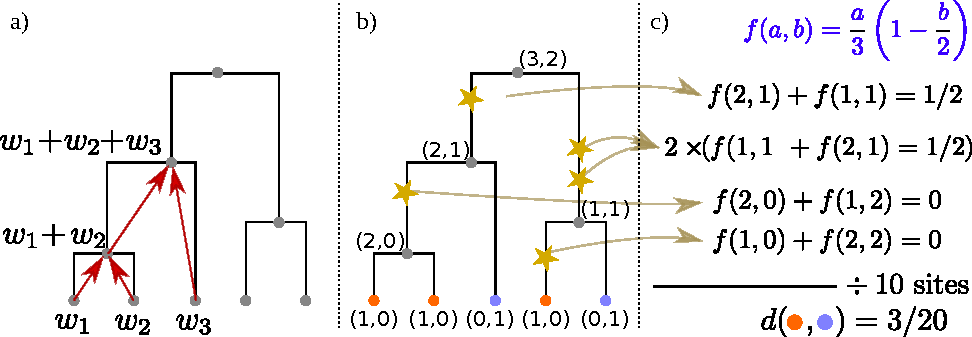
\includegraphics[width=\textwidth]{divergence_diagram}

}


%%%%%%%%%%%%%%%%%%%%%%%%%%%%%%%%%%%%%%%%%%%%%%%%%%%%%%%%%%%%%%%%%%%%%%%%%%%%%%
\headerbox{Duality}{name=duality,column=2,below=computation}{
%%%%%%%%%%%%%%%%%%%%%%%%%%%%%%%%%%%%%%%%%%%%%%%%%%%%%%%%%%%%%%%%%%%%%%%%%%%%%%

    Under infinite-site mutation at rate $\mu$,
\begin{align}
    \mu \branch(f, \iw)_{[i,j)}
    =
    \E\left[ \site(f, \iw)_{[i,j)} \given \treeseq_{[i,j)} \right] ,
\end{align}
and
\begin{align*}
    \var[\site(f, \iw)_{[i,j)}] 
    % &\qquad{}=
    %     \var\left[ \E\left[\site(f, \iw)_{[i,j)} \given \treeseq_{[i,j)}\right] \right]
    %     \\ & \qquad {}
    %         +
    %     \E\left[ \var\left[\site(f, \iw)_{[i,j)} \given \treeseq_{[i,j)}\right] \right]
    %     \\
    &=
        \mu^2 \var\left[ \branch(f, \iw)_{[i,j)} \right]
        \\ & \qquad {}
            +
        \frac{\mu}{j-i} \E\left[ \branch(f^2, \iw)_{[i,j)} \right] .
\end{align*}

After a few selective sweeps:

\includegraphics[width=\textwidth]{{swept.1000.999.1e-09.diversity.sub}.pdf}

\textbf{Real data:} 1000 Genomes tree sequences from Relate (Speidel et al 2019):

\includegraphics[width=\textwidth]{{relate_chr20_site_div_branch.1000000.diversity.mod}.pdf}
}
%%%%%%%%%%%%%%%%%%%%%%%%%%%%%%%%%%%%%%%%%%%%%%%%%%%%%%%%%%%%%%%%%%%%%%%%%%%%%%


%%%%%%%%%%%%%%%%%%%%%%%%%%%%%%%%%%%%%%%%%%%%%%%%%%%%%%%%%%%%%%%%%%%%%%%%%%%%%%
\headerbox{}{name=trees,column=0,above=bottom,span=3}{
%%%%%%%%%%%%%%%%%%%%%%%%%%%%%%%%%%%%%%%%%%%%%%%%%%%%%%%%%%%%%%%%%%%%%%%%%%%%%%

    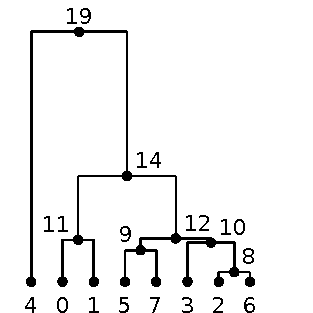
\includegraphics[width=0.085\textwidth]{tree0}
    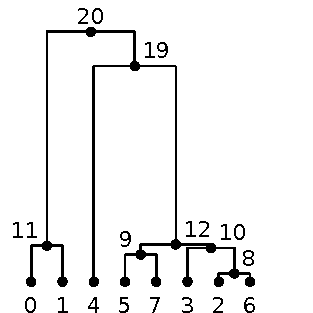
\includegraphics[width=0.085\textwidth]{tree1}
    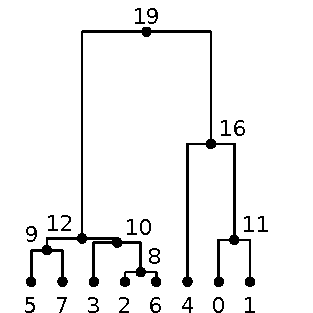
\includegraphics[width=0.085\textwidth]{tree2}
    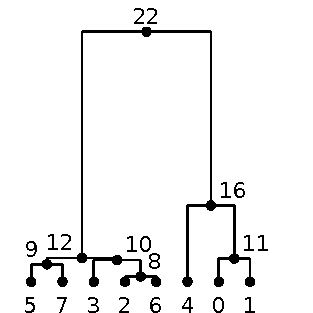
\includegraphics[width=0.085\textwidth]{tree3}
    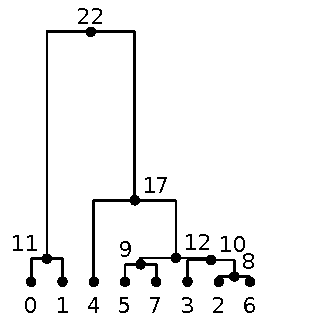
\includegraphics[width=0.085\textwidth]{tree4}
    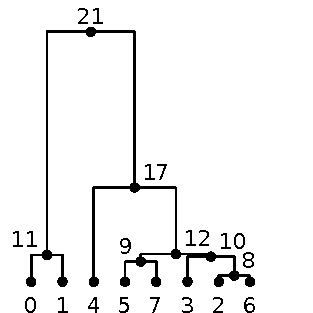
\includegraphics[width=0.085\textwidth]{tree5}
    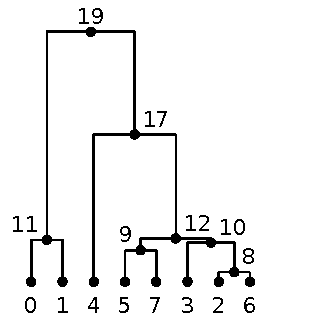
\includegraphics[width=0.085\textwidth]{tree6}
    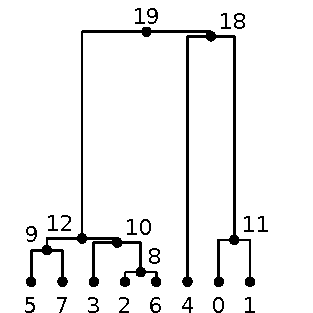
\includegraphics[width=0.085\textwidth]{tree7}
    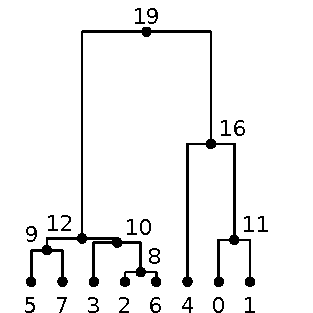
\includegraphics[width=0.085\textwidth]{tree8}
    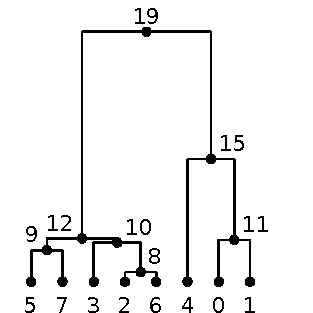
\includegraphics[width=0.085\textwidth]{tree9}
    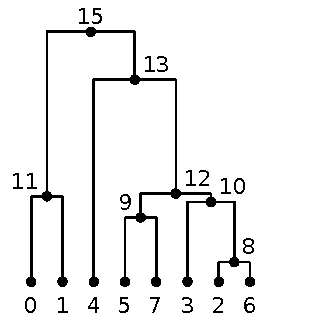
\includegraphics[width=0.085\textwidth]{tree10}


}
%%%%%%%%%%%%%%%%%%%%%%%%%%%%%%%%%%%%%%%%%%%%%%%%%%%%%%%%%%%%%%%%%%%%%%%%%%%%%%

\end{poster}%
\end{document}
